%% example.tex
%% Copyright 2012 Bruno Menegola
%
% This work may be distributed and/or modified under the
% conditions of the LaTeX Project Public License, either version 1.3
% of this license or (at your option) any later version.
% The latest version of this license is in
%   http://www.latex-project.org/lppl.txt
% and version 1.3 or later is part of all distributions of LaTeX
% version 2005/12/01 or later.
%
% This work has the LPPL maintenance status ‘maintained’.
%
% The Current Maintainer of this work is Bruno Menegola.
%
% This work consists of all files listed in MANIFEST
%
%
% Description
% ===========
%
% This is an example latex document to build presentation slides based on
% the beamer class using the Inf theme.

\documentclass{beamer}

\usepackage[T1]{fontenc}
\usepackage[english]{babel}
\usepackage[utf8]{inputenc}
\usepackage{tabularx}
\usepackage{ragged2e}
\usepackage{graphicx}
\usepackage{pgfplots}
\usepackage{xcolor}

%\usepackage{bibentry}

\definecolor{orange}{RGB}{230, 159, 0}
\definecolor{skyblue}{RGB}{86, 180, 233}
\definecolor{purple}{RGB}{204, 121, 167}
\definecolor{red}{RGB}{228, 26, 28}
\definecolor{green}{RGB}{166, 216, 84}
\definecolor{bluish}{RGB}{102,194,165}
\definecolor{white}{RGB}{255,255,255}
\definecolor{grey}{RGB}{128,128,128}
\definecolor{roboticsred}{RGB}{255, 22, 0}
\definecolor{roboticsgreen}{RGB}{56, 159, 0}
\definecolor{roboticsblue}{RGB}{86, 180, 233}

\pgfplotsset{
	precision recall color/.style={
		width=\textwidth, 
		height=\textwidth,
		grid=major,
		grid style={dashed, gray!30},
		xtick={0, 0.2, 0.4, 0.6, 0.8, 1},
		xlabel near ticks,
		xlabel=Recall,
		xlabel style={font=\footnotesize},
		ytick={0, 0.2, 0.4, 0.6, 0.8, 1},
		ylabel=Precision,
		ylabel style={font=\footnotesize, yshift=-0.3cm},		
		legend style={font=\tiny},
		legend cell align={left},
		cycle list={
			{color=bluish, line width=1pt, mark=none, mark options={line width=1pt, draw=bluish, fill=bluish, scale=1.5}},
			{color=green, line width=1pt, mark=none, mark options={line width=1pt, draw=green, fill=green, scale=1.5}},
			{color=red, line width=1pt, mark=none, mark options={line width=1pt, draw=red, fill=red, scale=1.5}},								
		}
	}
}

\pgfplotsset{
	precision recall/.style={
		width=0.55\columnwidth, 
		height=0.55\columnwidth,
		grid=major,
		grid style={dashed, gray!30},
		xtick={0, 0.2, 0.4, 0.6, 0.8, 1},
		xlabel near ticks,
		xlabel=Recall,
		xlabel style={font=\normalsize},
		ytick={0, 0.2, 0.4, 0.6, 0.8, 1},
		ylabel near ticks,
		ylabel=Precision,	
		ylabel style={font=\normalsize},		
		legend style={font=\normalsize},
		legend image post style={scale=0.3},
		cycle list={
			{color=orange, line width=1pt, mark=none, mark options={line width=1pt, draw=orange, fill=orange, scale=1.5}},
			{color=purple, line width=1pt, mark=none, mark options={line width=1pt, draw=purple, fill=purple, scale=1.5}},
			{color=skyblue, line width=1pt, mark=none, mark options={line width=1pt, draw=skyblue, fill=skyblue, scale=1.5}},								
		}
	}
}

% Choose the Inf theme
\usetheme{Inf}

\begin{document}

\setbeamertemplate{caption}{\raggedright\insertcaption\par}
\setbeamertemplate{footline}{}
% Define the title with \title[short title]{long title}
% Short title is optional
\title[]{\MakeLowercase{c}-M2DP: A Fast Point Cloud Descriptor with Color Information to Perform Loop Closure Detection}

% Optional subtitle
%\subtitle{Congresso XYZ}

\date{August, 2019}

% Author information
\author{\small Leonardo Perdomo, Diego Pittol \\ Mathias Mantelli, Renan Maffei \\ Mariana Kolberg and Edson Prestes}
\institute{Instituto de Informática --- UFRGS}



% Command to create title page
\InfTitlePage

\setbeamertemplate{footline}{\raisebox{9pt}{%
		\makebox[\paperwidth]{%
			\scriptsize\hfill\insertframenumber/\inserttotalframenumber\hspace{6pt}
		}
	}}

\section{Introduction}
\frame{
	\frametitle{Motivation}
	%\frametitle{Why 3D vision with color?}
	\begin{columns}
		\begin{column}{0.5\textwidth}
			%\begin{itemize}
				%\justifying
				%\item A 3D vision-based approach that uses color information:
				\begin{itemize}
					\justifying
					\item 3D spatial data can provide more descriptive scenes than only 2D images;
					%\item Spatial data with color can provide very descriptive scenes;
					\item Color can increase 3D descriptiveness\footnote[frame]{\tiny Tombari, Salti \& Stefano (2011), Feng, Liu \& Liao (2015), Logoglu, Kalkan \& Temizel (2016)}, but is insufficiently investigated for loop closure detection;
					%\item Color can increase descriptiveness, as reported in surface matching works\footnote[frame]{\tiny \cite{cshot2011,loind2015,cospair2016}};
					%\item Color can increase descriptiveness, as reported in surface matching works\footnote[frame]{\tiny \cite{cshot2011,loind2015,cospair2016}};
					%\item Considered less mature\footnote[frame]{\tiny \cite{m2dp2016, segmatch2017}} in relation to 2D approaches;
					\item Availability in recent benchmark platforms\footnote[frame]{\tiny Pandey, McBride \& Eustice (2011), Geiger, Lenz \& Urtasun (2012)}.
					%\item Color is often available alongside 3D data in recent benchmark platforms\footnote[frame]{\tiny \cite{fordcampus2011, kitti2012}}.
				%\end{itemize}   
			\end{itemize}
		\end{column}
		\begin{column}{0.5\textwidth}  %%<--- here
			\begin{center}
				\begin{figure}[h!]
					\centering
					%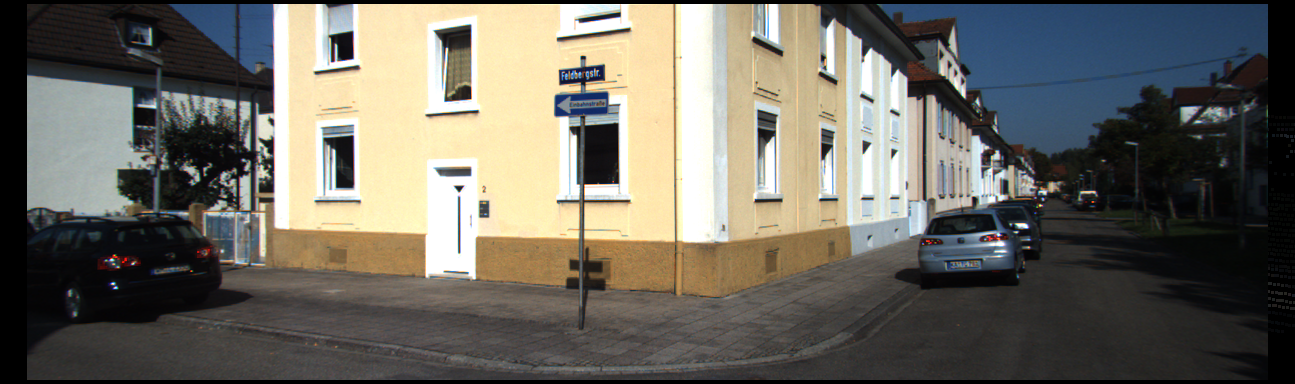
\includegraphics[scale=0.35, height=40pt, width=110pt]{1_419rgb.png}
					
					%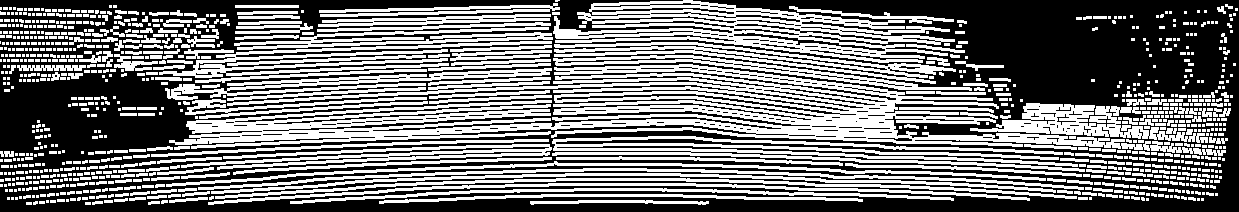
\includegraphics[scale=0.35, height=50pt, width=110pt]{2_419lidar2.png}
					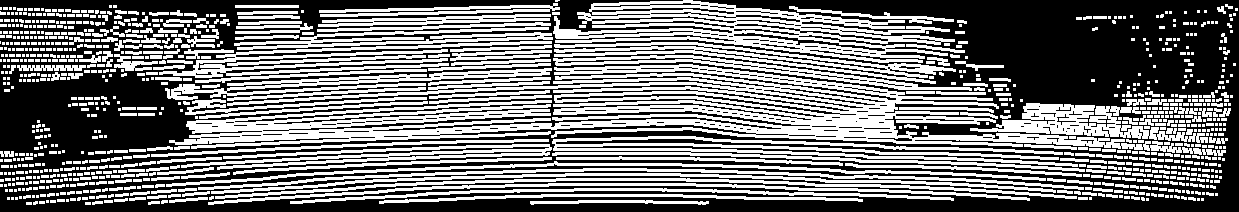
\includegraphics[scale=0.35, height=50pt, width=\textwidth]{2_419lidar2.png}
					
					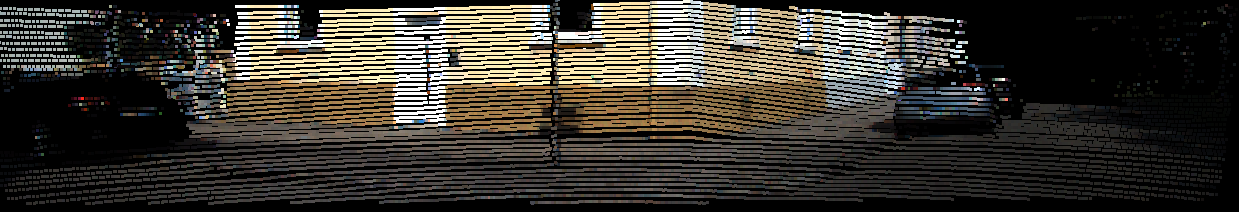
\includegraphics[scale=0.35, height=50pt, width=\textwidth]{3_419lidarcamera2.png}
					%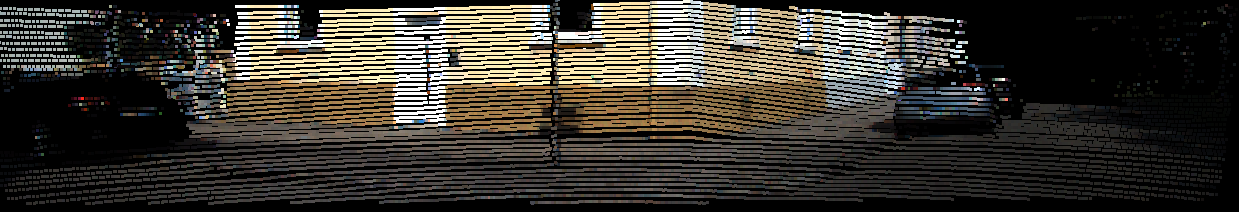
\includegraphics[scale=0.35, height=50pt, width=110pt]{3_419lidarcamera2.png}
					
					\caption{\centering \footnotesize Colored point cloud generated using LIDAR and camera.}
					\label{fig:pointclouds}
				\end{figure}
			\end{center}
		\end{column}
	\end{columns}  
}

\frame{
	\frametitle{Proposal}
	\begin{itemize}
		\justifying
		%\item We noticed that the M2DP descriptor can be extended to incorporate color data:
		%\item The main contributions of this work are: an extension of the state-of-the-art M2DP descriptor
		%\item Appearance signatures can be computed using shape, color, texture and other available data;
		%\begin{itemize}
			%\justifying
			%\item We noticed that the M2DP descriptor can be extended to incorporate color data in order to increase its descriptiveness.
			\item Color M2DP (c-M2DP), a global descriptor comprising of color and shape data computed from the point cloud:
			\begin{itemize}
				\justifying
				\item Takes advantage of M2DP's structure, extending it to compute color signatures from multiple 2D projections;
			\end{itemize}
			\item An improved loop closure detection, using the c-M2DP descriptor on point cloud sequences generated through camera-LIDAR fusion, or stereo depth estimation.
		%\end{itemize}
	\end{itemize}
}

\section{c-M2DP Descriptor}
\frame{
	\frametitle{Reference Frame}
	\begin{itemize}
		\justifying
		\item Rotation and shift invariance in 3D space;
		\item Point cloud $\boldsymbol{P}$ centroid is computed and used as the reference frame origin;
		\item PCA is performed on $\boldsymbol{P}$, with both the 1st and 2nd principal components defined as the $x$-axis and $y$-axis, respectively.
	\end{itemize}
}

\frame{
	\frametitle{Multiple 2D Projections}
	\begin{columns}
		\begin{column}{0.5\textwidth}
			\begin{itemize}
			\justifying
			\item A 2D plane $X$ is defined with normal vector $\boldsymbol{m}$ and $[\theta, \phi]$ parameters, which are used to generate distinct 2D planes;
			\item  $\boldsymbol{P}$ is projected onto each 2D plane, in order to compute shape and color signatures from each 2D projection.
			\end{itemize}
		\end{column}
		\begin{column}{0.5\textwidth}  %%<--- here
			\begin{center}
				\begin{figure}[h!]
					\centering
					\vspace{-1em}
					\begin{tikzpicture}[x=0.75pt,y=0.75pt,yscale=-0.6,xscale=0.6]
%uncomment if require: \path (0,300); %set diagram left start at 0, and has height of 300

%Image [id:dp09254054009459467] 
\draw (94.52,11.18) node  {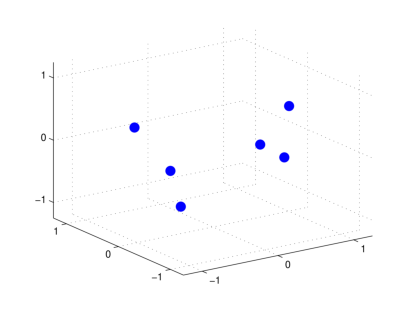
\includegraphics[width=79pt,height=70pt]{pointcloud.pdf}};
%Image [id:dp26150135761132864] 
\draw (15.52,166.18) node  {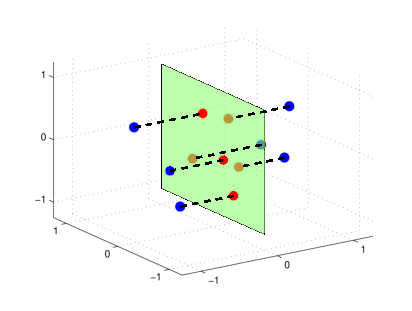
\includegraphics[width=79pt,height=70pt]{projection1.pdf}};
%Image [id:dp6062331233282552] 
\draw (192.52,166.18) node  {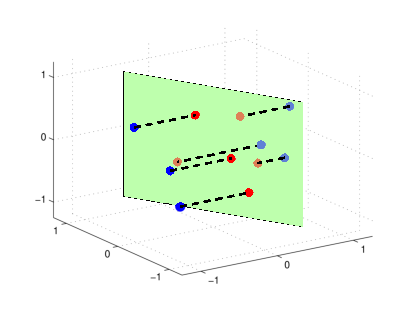
\includegraphics[width=79pt,height=70pt]{projection2.pdf}};
%Down Arrow [id:dp6057459970471565] 
\draw   (77,99.95) -- (84.51,99.95) -- (84.51,89.37) -- (115.52,89.37) -- (115.52,99.95) -- (120.03,99.95) -- (99.02,110) -- cycle ;

% Text Node
\draw (99.75,168.41) node  [align=left, scale=1.2] {\dots};


\end{tikzpicture}

					\vspace{-2em}
					\caption{\centering \footnotesize Projecting a point cloud $\boldsymbol{P}$ on multiple 2D planes.}
					\label{fig:multiple-projections}	
				\end{figure}
			\end{center}
		\end{column}
	\end{columns}	
}

\frame{
	\frametitle{Shape Signature}
	\begin{columns}
		\begin{column}{0.5\textwidth}
			\begin{itemize}
				\justifying
				\item Each plane is split into $l$ concentric circles  with varying radii $[r, 2^2r, \dots, l^2r]$;
				\item Each concentric circle is divided in $t$ shape bins, indexed by the $x$-axis; 
				\item Shape signature $\boldsymbol{s}_X$ is computed by counting the points within each bin.
			\end{itemize}
		\end{column}
		\begin{column}{0.5\textwidth}  %%<--- here
			\begin{center}
				\begin{figure}[h!]
					\centering
					\vspace{0.7cm}
					%\includegraphics[height=7cm]{shapesignature2.pdf}
					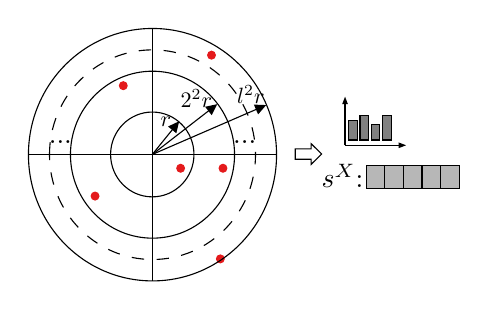
\begin{tikzpicture}[x=0.75pt,y=0.75pt,yscale=-0.6,xscale=0.6]
%uncomment if require: \path (0,388); %set diagram left start at 0, and has height of 388

%Shape: Ellipse [id:dp7382617193591512] 
\draw   (78.77,111.59) .. controls (78.77,92.78) and (93.76,77.53) .. (112.24,77.53) .. controls (130.73,77.53) and (145.71,92.78) .. (145.71,111.59) .. controls (145.71,130.4) and (130.73,145.64) .. (112.24,145.64) .. controls (93.76,145.64) and (78.77,130.4) .. (78.77,111.59) -- cycle ;
%Shape: Ellipse [id:dp25517697407182616] 
\draw   (46.54,111.77) .. controls (46.54,74.75) and (76.03,44.74) .. (112.42,44.74) .. controls (148.8,44.74) and (178.3,74.75) .. (178.3,111.77) .. controls (178.3,148.79) and (148.8,178.8) .. (112.42,178.8) .. controls (76.03,178.8) and (46.54,148.79) .. (46.54,111.77) -- cycle ;
%Shape: Ellipse [id:dp3459858941325883] 
\draw  [dash pattern={on 4.5pt off 4.5pt}] (29.7,111.77) .. controls (29.7,65.29) and (66.73,27.6) .. (112.42,27.6) .. controls (158.1,27.6) and (195.14,65.29) .. (195.14,111.77) .. controls (195.14,158.25) and (158.1,195.94) .. (112.42,195.94) .. controls (66.73,195.94) and (29.7,158.25) .. (29.7,111.77) -- cycle ;
%Shape: Ellipse [id:dp06494650200316232] 
\draw  [color={rgb, 255:red, 255; green, 0; blue, 0 }  ,draw opacity=1 ][fill={rgb, 255:red, 255; green, 0; blue, 0 }  ,fill opacity=1 ] (131.9,122.66) .. controls (131.9,120.92) and (133.29,119.51) .. (135,119.51) .. controls (136.72,119.51) and (138.11,120.92) .. (138.11,122.66) .. controls (138.11,124.41) and (136.72,125.82) .. (135,125.82) .. controls (133.29,125.82) and (131.9,124.41) .. (131.9,122.66) -- cycle ;
%Shape: Ellipse [id:dp0022695334650385535] 
\draw  [color={rgb, 255:red, 255; green, 0; blue, 0 }  ,draw opacity=1 ][fill={rgb, 255:red, 255; green, 0; blue, 0 }  ,fill opacity=1 ] (165.9,122.66) .. controls (165.9,120.92) and (167.29,119.51) .. (169.01,119.51) .. controls (170.72,119.51) and (172.11,120.92) .. (172.11,122.66) .. controls (172.11,124.41) and (170.72,125.82) .. (169.01,125.82) .. controls (167.29,125.82) and (165.9,124.41) .. (165.9,122.66) -- cycle ;
%Shape: Ellipse [id:dp9477076352826888] 
\draw  [color={rgb, 255:red, 255; green, 0; blue, 0 }  ,draw opacity=1 ][fill={rgb, 255:red, 255; green, 0; blue, 0 }  ,fill opacity=1 ] (85.85,56.36) .. controls (85.85,54.61) and (87.24,53.2) .. (88.96,53.2) .. controls (90.67,53.2) and (92.06,54.61) .. (92.06,56.36) .. controls (92.06,58.1) and (90.67,59.51) .. (88.96,59.51) .. controls (87.24,59.51) and (85.85,58.1) .. (85.85,56.36) -- cycle ;
%Shape: Ellipse [id:dp34247701706686684] 
\draw  [color={rgb, 255:red, 255; green, 0; blue, 0 }  ,draw opacity=1 ][fill={rgb, 255:red, 255; green, 0; blue, 0 }  ,fill opacity=1 ] (156.69,31.85) .. controls (156.69,30.11) and (158.08,28.69) .. (159.8,28.69) .. controls (161.51,28.69) and (162.9,30.11) .. (162.9,31.85) .. controls (162.9,33.59) and (161.51,35.01) .. (159.8,35.01) .. controls (158.08,35.01) and (156.69,33.59) .. (156.69,31.85) -- cycle ;
%Shape: Ellipse [id:dp5637425041894341] 
\draw  [color={rgb, 255:red, 255; green, 0; blue, 0 }  ,draw opacity=1 ][fill={rgb, 255:red, 255; green, 0; blue, 0 }  ,fill opacity=1 ] (63.19,145.01) .. controls (63.19,143.26) and (64.58,141.85) .. (66.29,141.85) .. controls (68.01,141.85) and (69.4,143.26) .. (69.4,145.01) .. controls (69.4,146.75) and (68.01,148.17) .. (66.29,148.17) .. controls (64.58,148.17) and (63.19,146.75) .. (63.19,145.01) -- cycle ;
%Shape: Ellipse [id:dp3859458151744748] 
\draw  [color={rgb, 255:red, 255; green, 0; blue, 0 }  ,draw opacity=1 ][fill={rgb, 255:red, 255; green, 0; blue, 0 }  ,fill opacity=1 ] (163.78,195.46) .. controls (163.78,193.72) and (165.17,192.3) .. (166.88,192.3) .. controls (168.6,192.3) and (169.99,193.72) .. (169.99,195.46) .. controls (169.99,197.21) and (168.6,198.62) .. (166.88,198.62) .. controls (165.17,198.62) and (163.78,197.21) .. (163.78,195.46) -- cycle ;
%Straight Lines [id:da9093409121292956] 
\draw    (112.24,10.23) -- (112.24,212.94) ;


%Straight Lines [id:da6639286505692693] 
\draw    (12.63,111.59) -- (211.86,111.59) ;


%Straight Lines [id:da5044264629099462] 
\draw    (112.24,111.59) -- (132.58,86.46) ;
\draw [shift={(133.84,84.91)}, rotate = 488.99] [fill={rgb, 255:red, 0; green, 0; blue, 0 }  ][line width=0.75]  [draw opacity=0] (8.93,-4.29) -- (0,0) -- (8.93,4.29) -- cycle    ;

%Straight Lines [id:da8524918674228583] 
\draw    (112.24,111.59) -- (162.79,72.44) ;
\draw [shift={(164.38,71.21)}, rotate = 502.25] [fill={rgb, 255:red, 0; green, 0; blue, 0 }  ][line width=0.75]  [draw opacity=0] (8.93,-4.29) -- (0,0) -- (8.93,4.29) -- cycle    ;

%Straight Lines [id:da5923697154582754] 
\draw    (112.24,111.59) -- (201.87,72.73) ;
\draw [shift={(203.71,71.94)}, rotate = 516.56] [fill={rgb, 255:red, 0; green, 0; blue, 0 }  ][line width=0.75]  [draw opacity=0] (8.93,-4.29) -- (0,0) -- (8.93,4.29) -- cycle    ;

%Shape: Ellipse [id:dp29860030053778785] 
\draw   (12.8,111.77) .. controls (12.8,55.79) and (57.4,10.41) .. (112.42,10.41) .. controls (167.43,10.41) and (212.03,55.79) .. (212.03,111.77) .. controls (212.03,167.75) and (167.43,213.13) .. (112.42,213.13) .. controls (57.4,213.13) and (12.8,167.75) .. (12.8,111.77) -- cycle ;
%Straight Lines [id:da0859952554415816] 
\draw    (267.03,104.23) -- (267.03,67.23) ;
\draw [shift={(267.03,65.23)}, rotate = 450] [fill={rgb, 255:red, 0; green, 0; blue, 0 }  ][line width=0.75]  [draw opacity=0] (5.93,-2.29) -- (0,0) -- (5.93,2.29) -- cycle    ;

%Straight Lines [id:da02894773929564054] 
\draw    (267.03,104.23) -- (314.03,104.23) ;
\draw [shift={(316.03,104.23)}, rotate = 180] [fill={rgb, 255:red, 0; green, 0; blue, 0 }  ][line width=0.75]  [draw opacity=0] (5.93,-2.29) -- (0,0) -- (5.93,2.29) -- cycle    ;

%Shape: Rectangle [id:dp6434985742147902] 
\draw  [color=black  ,draw opacity=1 ][fill=grey  ,fill opacity=1 ] (270.03,84.23) -- (277.03,84.23) -- (277.03,100) -- (270.03,100) -- cycle ;
%Shape: Rectangle [id:dp9582021838782706] 
\draw  [color=black  ,draw opacity=1 ][fill=grey  ,fill opacity=1 ] (279.03,80.23) -- (286.03,80.23) -- (286.03,100) -- (279.03,100) -- cycle ;
%Shape: Rectangle [id:dp6964465553467404] 
\draw  [color=black  ,draw opacity=1 ][fill=grey  ,fill opacity=1 ] (288.03,87.23) -- (295.03,87.23) -- (295.03,100) -- (288.03,100) -- cycle ;
%Shape: Rectangle [id:dp8568290678115581] 
\draw  [color=black  ,draw opacity=1 ][fill=grey  ,fill opacity=1 ] (297.03,80.23) -- (304.03,80.23) -- (304.03,100) -- (297.03,100) -- cycle ;


%Shape: Rectangle [id:dp12299147827719992] 
\draw  [fill=grey  ,fill opacity=0.57 ] (284,120.23) -- (298.77,120.23) -- (298.77,139.14) -- (284,139.14) -- cycle ;
%Shape: Rectangle [id:dp056770282484357115] 
\draw  [fill=grey  ,fill opacity=0.57 ] (299,120.23) -- (313.77,120.23) -- (313.77,139.14) -- (299,139.14) -- cycle ;
%Shape: Rectangle [id:dp8374236504797968] 
\draw  [fill=grey  ,fill opacity=0.57 ] (314,120.23) -- (328.77,120.23) -- (328.77,139.14) -- (314,139.14) -- cycle ;
%Shape: Rectangle [id:dp8517953159568432] 
\draw  [fill=grey  ,fill opacity=0.57 ] (329,120.23) -- (343.77,120.23) -- (343.77,139.14) -- (329,139.14) -- cycle ;
%Shape: Rectangle [id:dp797061078463292] 
\draw  [fill=grey  ,fill opacity=0.57 ] (344,120.23) -- (358.77,120.23) -- (358.77,139.14) -- (344,139.14) -- cycle ;

%Down Arrow [id:dp7628921897948798] 
\draw   (239.75,119.59) -- (239.75,115.41) -- (227.03,115.41) -- (227.03,107.05) -- (239.75,107.05) -- (239.75,102.88) -- (248.23,111.23) -- cycle ;


% Text Node
\draw (186.44,101.76) node  [scale=1] {...};
% Text Node
\draw (38.44,101.76) node  [scale=1] {...};
% Text Node
\draw (147.64,66.72) node [scale=0.8]  {$2^{2} r$};
% Text Node
\draw (123.27,85.46) node [scale=0.8]  {$r$};
% Text Node
\draw (191.43,63.12) node [scale=0.8]  {$l^{2} r$};
% Text Node
\draw (265,128.6) node   {$\boldsymbol{s}^{X}$:};

\end{tikzpicture}
					\caption{\centering \footnotesize Computing the shape signature $\boldsymbol{s}_X$.}
					\label{fig:shape-signature}	
				\end{figure}
			\end{center}
		\end{column}
	\end{columns}	
}

\frame{
	\frametitle{Color Signature}
	\begin{columns}
		\begin{column}{0.5\textwidth}
			\begin{itemize}
				\justifying
				\item For every concentric circle, histograms of the color channels, which are divided in $j$ bins, are computed;
				\item These histograms are concatenated them into a single color signature vector $\boldsymbol{c}_X$;
			\end{itemize}
		\end{column}
		\begin{column}{0.5\textwidth}  %%<--- here
			\begin{center}
				\begin{figure}[h!]
					\centering
					\vspace{0.7cm}
					%\includegraphics[height=7cm]{shapesignature2.pdf}
					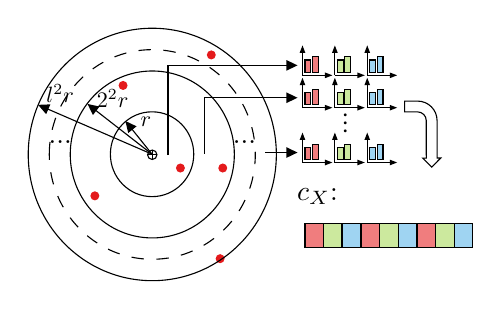
\begin{tikzpicture}[x=0.75pt,y=0.75pt,yscale=-0.6,xscale=0.6]
%uncomment if require: \path (0,300); %set diagram left start at 0, and has height of 300

%Shape: Ellipse [id:dp22042437585940766] 
\draw   (98.77,131.59) .. controls (98.77,112.78) and (113.76,97.53) .. (132.24,97.53) .. controls (150.73,97.53) and (165.71,112.78) .. (165.71,131.59) .. controls (165.71,150.4) and (150.73,165.64) .. (132.24,165.64) .. controls (113.76,165.64) and (98.77,150.4) .. (98.77,131.59) -- cycle ;
%Shape: Ellipse [id:dp5949676512076546] 
\draw   (66.54,131.77) .. controls (66.54,94.75) and (96.03,64.74) .. (132.42,64.74) .. controls (168.8,64.74) and (198.3,94.75) .. (198.3,131.77) .. controls (198.3,168.79) and (168.8,198.8) .. (132.42,198.8) .. controls (96.03,198.8) and (66.54,168.79) .. (66.54,131.77) -- cycle ;
%Shape: Ellipse [id:dp7072370567814422] 
\draw  [dash pattern={on 4.5pt off 4.5pt}] (49.7,131.77) .. controls (49.7,85.29) and (86.73,47.6) .. (132.42,47.6) .. controls (178.1,47.6) and (215.14,85.29) .. (215.14,131.77) .. controls (215.14,178.25) and (178.1,215.94) .. (132.42,215.94) .. controls (86.73,215.94) and (49.7,178.25) .. (49.7,131.77) -- cycle ;
%Shape: Ellipse [id:dp9376040493166226] 
\draw  [color={rgb, 255:red, 255; green, 0; blue, 0 }  ,draw opacity=1 ][fill={rgb, 255:red, 255; green, 0; blue, 0 }  ,fill opacity=1 ] (151.9,142.66) .. controls (151.9,140.92) and (153.29,139.51) .. (155,139.51) .. controls (156.72,139.51) and (158.11,140.92) .. (158.11,142.66) .. controls (158.11,144.41) and (156.72,145.82) .. (155,145.82) .. controls (153.29,145.82) and (151.9,144.41) .. (151.9,142.66) -- cycle ;
%Shape: Ellipse [id:dp6728764854992865] 
\draw  [color={rgb, 255:red, 255; green, 0; blue, 0 }  ,draw opacity=1 ][fill={rgb, 255:red, 255; green, 0; blue, 0 }  ,fill opacity=1 ] (185.9,142.66) .. controls (185.9,140.92) and (187.29,139.51) .. (189.01,139.51) .. controls (190.72,139.51) and (192.11,140.92) .. (192.11,142.66) .. controls (192.11,144.41) and (190.72,145.82) .. (189.01,145.82) .. controls (187.29,145.82) and (185.9,144.41) .. (185.9,142.66) -- cycle ;
%Shape: Ellipse [id:dp1494936101048986] 
\draw  [color={rgb, 255:red, 255; green, 0; blue, 0 }  ,draw opacity=1 ][fill={rgb, 255:red, 255; green, 0; blue, 0 }  ,fill opacity=1 ] (105.85,76.36) .. controls (105.85,74.61) and (107.24,73.2) .. (108.96,73.2) .. controls (110.67,73.2) and (112.06,74.61) .. (112.06,76.36) .. controls (112.06,78.1) and (110.67,79.51) .. (108.96,79.51) .. controls (107.24,79.51) and (105.85,78.1) .. (105.85,76.36) -- cycle ;
%Shape: Ellipse [id:dp5546182167747219] 
\draw  [color={rgb, 255:red, 255; green, 0; blue, 0 }  ,draw opacity=1 ][fill={rgb, 255:red, 255; green, 0; blue, 0 }  ,fill opacity=1 ] (176.69,51.85) .. controls (176.69,50.11) and (178.08,48.69) .. (179.8,48.69) .. controls (181.51,48.69) and (182.9,50.11) .. (182.9,51.85) .. controls (182.9,53.59) and (181.51,55.01) .. (179.8,55.01) .. controls (178.08,55.01) and (176.69,53.59) .. (176.69,51.85) -- cycle ;
%Shape: Ellipse [id:dp20582881370354322] 
\draw  [color={rgb, 255:red, 255; green, 0; blue, 0 }  ,draw opacity=1 ][fill={rgb, 255:red, 255; green, 0; blue, 0 }  ,fill opacity=1 ] (83.19,165.01) .. controls (83.19,163.26) and (84.58,161.85) .. (86.29,161.85) .. controls (88.01,161.85) and (89.4,163.26) .. (89.4,165.01) .. controls (89.4,166.75) and (88.01,168.17) .. (86.29,168.17) .. controls (84.58,168.17) and (83.19,166.75) .. (83.19,165.01) -- cycle ;
%Shape: Ellipse [id:dp35339284724607267] 
\draw  [color={rgb, 255:red, 255; green, 0; blue, 0 }  ,draw opacity=1 ][fill={rgb, 255:red, 255; green, 0; blue, 0 }  ,fill opacity=1 ] (183.78,215.46) .. controls (183.78,213.72) and (185.17,212.3) .. (186.88,212.3) .. controls (188.6,212.3) and (189.99,213.72) .. (189.99,215.46) .. controls (189.99,217.21) and (188.6,218.62) .. (186.88,218.62) .. controls (185.17,218.62) and (183.78,217.21) .. (183.78,215.46) -- cycle ;
%Straight Lines [id:da8440305272338511] 
\draw    (132.38,128.23) -- (132.38,135.8) ;


%Straight Lines [id:da18353521910609616] 
\draw    (128.6,132.02) -- (136.16,132.02) ;


%Straight Lines [id:da6160021318684068] 
\draw    (132.24,131.59) -- (112.09,106.47) ;
\draw [shift={(110.84,104.91)}, rotate = 411.26] [fill={rgb, 255:red, 0; green, 0; blue, 0 }  ][line width=0.75]  [draw opacity=0] (8.93,-4.29) -- (0,0) -- (8.93,4.29) -- cycle    ;

%Straight Lines [id:da4361175020790148] 
\draw    (132.24,131.59) -- (81.95,92.44) ;
\draw [shift={(80.38,91.21)}, rotate = 397.9] [fill={rgb, 255:red, 0; green, 0; blue, 0 }  ][line width=0.75]  [draw opacity=0] (8.93,-4.29) -- (0,0) -- (8.93,4.29) -- cycle    ;

%Straight Lines [id:da2816608379552582] 
\draw    (132.24,131.59) -- (42.54,92.73) ;
\draw [shift={(40.71,91.94)}, rotate = 383.41999999999996] [fill={rgb, 255:red, 0; green, 0; blue, 0 }  ][line width=0.75]  [draw opacity=0] (8.93,-4.29) -- (0,0) -- (8.93,4.29) -- cycle    ;

%Shape: Ellipse [id:dp6312040354242004] 
\draw   (32.8,131.77) .. controls (32.8,75.79) and (77.4,30.41) .. (132.42,30.41) .. controls (187.43,30.41) and (232.03,75.79) .. (232.03,131.77) .. controls (232.03,187.75) and (187.43,233.13) .. (132.42,233.13) .. controls (77.4,233.13) and (32.8,187.75) .. (32.8,131.77) -- cycle ;
%Straight Lines [id:da7388753114522317] 
\draw    (253.03,68.23) -- (253.03,46.23) ;
\draw [shift={(253.03,44.23)}, rotate = 450] [fill={rgb, 255:red, 0; green, 0; blue, 0 }  ][line width=0.75]  [draw opacity=0] (5.93,-2.29) -- (0,0) -- (5.93,2.29) -- cycle    ;

%Straight Lines [id:da4000394565086268] 
\draw    (253.03,68.23) -- (275.03,68.23) ;
\draw [shift={(277.03,68.23)}, rotate = 180] [fill={rgb, 255:red, 0; green, 0; blue, 0 }  ][line width=0.75]  [draw opacity=0] (5.93,-2.29) -- (0,0) -- (5.93,2.29) -- cycle    ;

%Shape: Rectangle [id:dp016947909178976484] 
\draw  [color=black  ,draw opacity=1 ][fill=red  ,fill opacity=0.57 ] (255.03,55.93) -- (259.7,55.93) -- (259.7,65.63) -- (255.03,65.63) -- cycle ;
%Shape: Rectangle [id:dp5625317123053011] 
\draw  [color=black  ,draw opacity=1 ][fill=red  ,fill opacity=0.57 ] (261.03,53.46) -- (265.7,53.46) -- (265.7,65.63) -- (261.03,65.63) -- cycle ;

%Straight Lines [id:da620614004914323] 
\draw    (145.03,132.23) -- (145.03,60.23) ;


%Shape: Circle [id:dp005683642466507988] 
\draw   (128.6,132.02) .. controls (128.6,129.93) and (130.29,128.23) .. (132.38,128.23) .. controls (134.47,128.23) and (136.16,129.93) .. (136.16,132.02) .. controls (136.16,134.11) and (134.47,135.8) .. (132.38,135.8) .. controls (130.29,135.8) and (128.6,134.11) .. (128.6,132.02) -- cycle ;
%Straight Lines [id:da022437387852998092] 
\draw    (145.03,60.23) -- (247.03,60.23) ;
\draw [shift={(249.03,60.23)}, rotate = 180] [fill={rgb, 255:red, 0; green, 0; blue, 0 }  ][line width=0.75]  [draw opacity=0] (8.93,-4.29) -- (0,0) -- (8.93,4.29) -- cycle    ;

%Straight Lines [id:da3327524132297772] 
\draw    (174.03,131.23) -- (174.03,86.23) ;


%Straight Lines [id:da2525359458205172] 
\draw    (279.03,68.23) -- (279.03,46.23) ;
\draw [shift={(279.03,44.23)}, rotate = 450] [fill={rgb, 255:red, 0; green, 0; blue, 0 }  ][line width=0.75]  [draw opacity=0] (5.93,-2.29) -- (0,0) -- (5.93,2.29) -- cycle    ;

%Straight Lines [id:da16414789555797105] 
\draw    (279.03,68.23) -- (301.03,68.23) ;
\draw [shift={(303.03,68.23)}, rotate = 180] [fill={rgb, 255:red, 0; green, 0; blue, 0 }  ][line width=0.75]  [draw opacity=0] (5.93,-2.29) -- (0,0) -- (5.93,2.29) -- cycle    ;

%Shape: Rectangle [id:dp8274809657348666] 
\draw  [color=black  ,draw opacity=1 ][fill=green  ,fill opacity=0.57 ] (281.03,55.93) -- (285.7,55.93) -- (285.7,65.63) -- (281.03,65.63) -- cycle ;
%Shape: Rectangle [id:dp06782765238071065] 
\draw  [color=black  ,draw opacity=1 ][fill=green  ,fill opacity=0.57 ] (287.03,53.46) -- (291.7,53.46) -- (291.7,65.63) -- (287.03,65.63) -- cycle ;
%Straight Lines [id:da04541867871992544] 
\draw    (305.03,68.23) -- (305.03,46.23) ;
\draw [shift={(305.03,44.23)}, rotate = 450] [fill={rgb, 255:red, 0; green, 0; blue, 0 }  ][line width=0.75]  [draw opacity=0] (5.93,-2.29) -- (0,0) -- (5.93,2.29) -- cycle    ;

%Straight Lines [id:da20964508840822693] 
\draw    (305.03,68.23) -- (327.03,68.23) ;
\draw [shift={(329.03,68.23)}, rotate = 180] [fill={rgb, 255:red, 0; green, 0; blue, 0 }  ][line width=0.75]  [draw opacity=0] (5.93,-2.29) -- (0,0) -- (5.93,2.29) -- cycle    ;

%Shape: Rectangle [id:dp6690668435039354] 
\draw  [color=black  ,draw opacity=1 ][fill=skyblue  ,fill opacity=0.57 ] (307.03,55.93) -- (311.7,55.93) -- (311.7,65.63) -- (307.03,65.63) -- cycle ;
%Shape: Rectangle [id:dp9255699869921165] 
\draw  [color=black  ,draw opacity=1 ][fill=skyblue  ,fill opacity=0.57 ] (313.03,53.46) -- (317.7,53.46) -- (317.7,65.63) -- (313.03,65.63) -- cycle ;
%Straight Lines [id:da8165440404194242] 
\draw    (253.03,94.23) -- (253.03,72.23) ;
\draw [shift={(253.03,70.23)}, rotate = 450] [fill={rgb, 255:red, 0; green, 0; blue, 0 }  ][line width=0.75]  [draw opacity=0] (5.93,-2.29) -- (0,0) -- (5.93,2.29) -- cycle    ;

%Straight Lines [id:da29454216862732807] 
\draw    (253.03,94.23) -- (275.03,94.23) ;
\draw [shift={(277.03,94.23)}, rotate = 180] [fill={rgb, 255:red, 0; green, 0; blue, 0 }  ][line width=0.75]  [draw opacity=0] (5.93,-2.29) -- (0,0) -- (5.93,2.29) -- cycle    ;

%Shape: Rectangle [id:dp2984155781668567] 
\draw  [color=black  ,draw opacity=1 ][fill=red  ,fill opacity=0.57 ] (255.03,81.93) -- (259.7,81.93) -- (259.7,91.63) -- (255.03,91.63) -- cycle ;
%Shape: Rectangle [id:dp7229599369299615] 
\draw  [color=black  ,draw opacity=1 ][fill=red  ,fill opacity=0.57 ] (261.03,79.46) -- (265.7,79.46) -- (265.7,91.63) -- (261.03,91.63) -- cycle ;
%Straight Lines [id:da10039448001605955] 
\draw    (279.03,94.23) -- (279.03,72.23) ;
\draw [shift={(279.03,70.23)}, rotate = 450] [fill={rgb, 255:red, 0; green, 0; blue, 0 }  ][line width=0.75]  [draw opacity=0] (5.93,-2.29) -- (0,0) -- (5.93,2.29) -- cycle    ;

%Straight Lines [id:da8722018166510564] 
\draw    (279.03,94.23) -- (301.03,94.23) ;
\draw [shift={(303.03,94.23)}, rotate = 180] [fill={rgb, 255:red, 0; green, 0; blue, 0 }  ][line width=0.75]  [draw opacity=0] (5.93,-2.29) -- (0,0) -- (5.93,2.29) -- cycle    ;

%Shape: Rectangle [id:dp5710893991029787] 
\draw  [color=black  ,draw opacity=1 ][fill=green  ,fill opacity=0.57 ] (281.03,81.93) -- (285.7,81.93) -- (285.7,91.63) -- (281.03,91.63) -- cycle ;
%Shape: Rectangle [id:dp9056928866973952] 
\draw  [color=black  ,draw opacity=1 ][fill=green  ,fill opacity=0.57 ] (287.03,79.46) -- (291.7,79.46) -- (291.7,91.63) -- (287.03,91.63) -- cycle ;
%Straight Lines [id:da48015611435891126] 
\draw    (305.03,94.23) -- (305.03,72.23) ;
\draw [shift={(305.03,70.23)}, rotate = 450] [fill={rgb, 255:red, 0; green, 0; blue, 0 }  ][line width=0.75]  [draw opacity=0] (5.93,-2.29) -- (0,0) -- (5.93,2.29) -- cycle    ;

%Straight Lines [id:da21508790577080394] 
\draw    (305.03,94.23) -- (327.03,94.23) ;
\draw [shift={(329.03,94.23)}, rotate = 180] [fill={rgb, 255:red, 0; green, 0; blue, 0 }  ][line width=0.75]  [draw opacity=0] (5.93,-2.29) -- (0,0) -- (5.93,2.29) -- cycle    ;

%Shape: Rectangle [id:dp656328402305677] 
\draw  [color=black  ,draw opacity=1 ][fill=skyblue  ,fill opacity=0.57 ] (307.03,81.93) -- (311.7,81.93) -- (311.7,91.63) -- (307.03,91.63) -- cycle ;
%Shape: Rectangle [id:dp5664134518061891] 
\draw  [color=black  ,draw opacity=1 ][fill=skyblue  ,fill opacity=0.57 ] (313.03,79.46) -- (317.7,79.46) -- (317.7,91.63) -- (313.03,91.63) -- cycle ;
%Straight Lines [id:da26856630441769913] 
\draw    (253.03,138.23) -- (253.03,116.23) ;
\draw [shift={(253.03,114.23)}, rotate = 450] [fill={rgb, 255:red, 0; green, 0; blue, 0 }  ][line width=0.75]  [draw opacity=0] (5.93,-2.29) -- (0,0) -- (5.93,2.29) -- cycle    ;

%Straight Lines [id:da045342033266806414] 
\draw    (253.03,138.23) -- (275.03,138.23) ;
\draw [shift={(277.03,138.23)}, rotate = 180] [fill={rgb, 255:red, 0; green, 0; blue, 0 }  ][line width=0.75]  [draw opacity=0] (5.93,-2.29) -- (0,0) -- (5.93,2.29) -- cycle    ;

%Shape: Rectangle [id:dp21465817035357382] 
\draw  [color=black  ,draw opacity=1][fill=red  ,fill opacity=0.57 ] (255.03,125.93) -- (259.7,125.93) -- (259.7,135.63) -- (255.03,135.63) -- cycle ;
%Shape: Rectangle [id:dp6836107840104558] 
\draw  [color=black  ,draw opacity=1][fill=red  ,fill opacity=0.57 ] (261.03,123.46) -- (265.7,123.46) -- (265.7,135.63) -- (261.03,135.63) -- cycle ;
%Straight Lines [id:da7152252219644601] 
\draw    (279.03,138.23) -- (279.03,116.23) ;
\draw [shift={(279.03,114.23)}, rotate = 450] [fill={rgb, 255:red, 0; green, 0; blue, 0 }  ][line width=0.75]  [draw opacity=0] (5.93,-2.29) -- (0,0) -- (5.93,2.29) -- cycle    ;

%Straight Lines [id:da9384291951491641] 
\draw    (279.03,138.23) -- (301.03,138.23) ;
\draw [shift={(303.03,138.23)}, rotate = 180] [fill={rgb, 255:red, 0; green, 0; blue, 0 }  ][line width=0.75]  [draw opacity=0] (5.93,-2.29) -- (0,0) -- (5.93,2.29) -- cycle    ;

%Shape: Rectangle [id:dp30291585437230484] 
\draw  [color=black  ,draw opacity=1][fill=green  ,fill opacity=0.57 ] (281.03,125.93) -- (285.7,125.93) -- (285.7,135.63) -- (281.03,135.63) -- cycle ;
%Shape: Rectangle [id:dp8268094585264629] 
\draw  [color=black  ,draw opacity=1][fill=green  ,fill opacity=0.57 ] (287.03,123.46) -- (291.7,123.46) -- (291.7,135.63) -- (287.03,135.63) -- cycle ;
%Straight Lines [id:da6298730087940589] 
\draw    (305.03,138.23) -- (305.03,116.23) ;
\draw [shift={(305.03,114.23)}, rotate = 450] [fill={rgb, 255:red, 0; green, 0; blue, 0 }  ][line width=0.75]  [draw opacity=0] (5.93,-2.29) -- (0,0) -- (5.93,2.29) -- cycle    ;

%Straight Lines [id:da3708666876743798] 
\draw    (305.03,138.23) -- (327.03,138.23) ;
\draw [shift={(329.03,138.23)}, rotate = 180] [fill={rgb, 255:red, 0; green, 0; blue, 0 }  ][line width=0.75]  [draw opacity=0] (5.93,-2.29) -- (0,0) -- (5.93,2.29) -- cycle    ;

%Shape: Rectangle [id:dp00038976604596641096] 
\draw  [color=black  ,draw opacity=1][fill=skyblue  ,fill opacity=0.57 ] (307.03,125.93) -- (311.7,125.93) -- (311.7,135.63) -- (307.03,135.63) -- cycle ;
%Shape: Rectangle [id:dp36800166267960555] 
\draw  [color=black  ,draw opacity=1][fill=skyblue  ,fill opacity=0.57 ] (313.03,123.46) -- (317.7,123.46) -- (317.7,135.63) -- (313.03,135.63) -- cycle ;
%Straight Lines [id:da7693768627138445] 
\draw    (174.03,86.23) -- (247.03,86.23) ;
\draw [shift={(249.03,86.23)}, rotate = 180] [fill={rgb, 255:red, 0; green, 0; blue, 0 }  ][line width=0.75]  [draw opacity=0] (8.93,-4.29) -- (0,0) -- (8.93,4.29) -- cycle    ;

%Straight Lines [id:da607729095409385] 
\draw    (223.03,130.23) -- (247.03,130.23) ;
\draw [shift={(249.03,130.23)}, rotate = 180] [fill={rgb, 255:red, 0; green, 0; blue, 0 }  ][line width=0.75]  [draw opacity=0] (8.93,-4.29) -- (0,0) -- (8.93,4.29) -- cycle    ;

%Shape: Rectangle [id:dp8711908392617309] 
\draw  [fill=red ,fill opacity=0.57 ] (255,187.23) -- (269.77,187.23) -- (269.77,206.14) -- (255,206.14) -- cycle ;
%Shape: Rectangle [id:dp18481612105128353] 
\draw  [fill=green  ,fill opacity=0.57 ] (270,187.23) -- (284.77,187.23) -- (284.77,206.14) -- (270,206.14) -- cycle ;
%Shape: Rectangle [id:dp7615959072987122] 
\draw  [fill=skyblue  ,fill opacity=0.57 ] (285,187.23) -- (299.77,187.23) -- (299.77,206.14) -- (285,206.14) -- cycle ;
%Shape: Rectangle [id:dp1813533709159073] 
\draw  [fill=red ,fill opacity=0.57 ] (300,187.23) -- (314.77,187.23) -- (314.77,206.14) -- (300,206.14) -- cycle ;
%Shape: Rectangle [id:dp8129375218164283] 
\draw  [fill=green  ,fill opacity=0.57 ] (315,187.23) -- (329.77,187.23) -- (329.77,206.14) -- (315,206.14) -- cycle ;
%Shape: Rectangle [id:dp9302976015184905] 
\draw  [fill=skyblue  ,fill opacity=0.57 ] (330,187.23) -- (344.77,187.23) -- (344.77,206.14) -- (330,206.14) -- cycle ;
%Shape: Rectangle [id:dp3052728377366358] 
\draw  [fill=red  ,fill opacity=0.57 ] (345,187.23) -- (359.77,187.23) -- (359.77,206.14) -- (345,206.14) -- cycle ;
%Shape: Rectangle [id:dp9806675697084216] 
\draw  [fill=green  ,fill opacity=0.57 ] (360,187.23) -- (374.77,187.23) -- (374.77,206.14) -- (360,206.14) -- cycle ;
%Shape: Rectangle [id:dp526916695713156] 
\draw  [fill=skyblue  ,fill opacity=0.57 ] (375,187.23) -- (389.77,187.23) -- (389.77,206.14) -- (375,206.14) -- cycle ;

%Bend Arrow [id:dp941959923921848] 
\draw   (335.03,88.93) -- (345.45,88.92) .. controls (354.07,88.91) and (361.08,95.89) .. (361.09,104.52) -- (361.13,134.65) -- (364.02,134.64) -- (356.8,141.94) -- (349.56,134.66) -- (352.45,134.66) -- (352.41,104.53) .. controls (352.41,100.7) and (349.29,97.59) .. (345.46,97.6) -- (335.05,97.61) -- cycle ;

% Text Node
\draw (206.44,121.76) node  [scale=1] {...};
% Text Node
\draw (58.44,121.76) node  [scale=1] {...};
% Text Node
\draw (100.64,86.72) node [scale=0.8]  {$2^{2} r$};
% Text Node
\draw (127.27,105.46) node [scale=0.8]  {$r$};
% Text Node
\draw (58.43,83.12) node [scale=0.8]  {$l^{2} r$};
% Text Node
\draw (287.44,106.76) node [rotate=-90] [align=left] {...};
% Text Node
\draw (265,165.6) node   {$\boldsymbol{c}_{X}$:};

\end{tikzpicture}

					\caption{\centering \footnotesize Computing the color signature $\boldsymbol{c}_X$.}
					\label{fig:color-signature}	
				\end{figure}
			\end{center}
		\end{column}
	\end{columns}	
}

\frame{
	\frametitle{Signature Vector}
	\begin{columns}
		\begin{column}{0.5\textwidth}
			\begin{itemize}
				\justifying
				\item Both $\boldsymbol{s}_X$ and $\boldsymbol{c}_X$ are normalized and concatenated into a single signature vector;
				\item The signature matrix $\boldsymbol{A}$ is augmented by a row with the concatenated vector.
			\end{itemize}
		\end{column}
		\begin{column}{0.5\textwidth}  %%<--- here
			\begin{center}
				\begin{figure}[h!]
					\centering
					\vspace{0.7cm}
					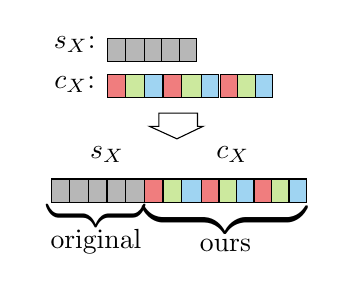
\begin{tikzpicture}[x=0.75pt,y=0.75pt,yscale=-0.6,xscale=0.6]
%uncomment if require: \path (0,300); %set diagram left start at 0, and has height of 300

%Shape: Rectangle [id:dp056770282484357115] 
\draw  [fill=grey  ,fill opacity=0.57 ] (133,39.23) -- (146.77,39.23) -- (146.77,58.14) -- (133,58.14) -- cycle ;
%Shape: Rectangle [id:dp8374236504797968] 
\draw  [fill=grey  ,fill opacity=0.57 ] (147,39.23) -- (160.77,39.23) -- (160.77,58.14) -- (147,58.14) -- cycle ;
%Shape: Rectangle [id:dp8517953159568432] 
\draw  [fill=grey  ,fill opacity=0.57 ] (161,39.23) -- (174.77,39.23) -- (174.77,58.14) -- (161,58.14) -- cycle ;
%Shape: Rectangle [id:dp797061078463292] 
\draw  [fill=grey  ,fill opacity=0.57 ] (103,39.23) -- (117.77,39.23) -- (117.77,58.14) -- (103,58.14) -- cycle ;
%Shape: Rectangle [id:dp12299147827719992] 
\draw  [fill=grey  ,fill opacity=0.57 ] (118,39.23) -- (132.77,39.23) -- (132.77,58.14) -- (118,58.14) -- cycle ;

%Shape: Rectangle [id:dp8711908392617309] 
\draw  [fill=red ,fill opacity=0.57 ] (194,68.23) -- (207.77,68.23) -- (207.77,87.14) -- (194,87.14) -- cycle ;
%Shape: Rectangle [id:dp18481612105128353] 
\draw  [fill=green  ,fill opacity=0.57 ] (208,68.23) -- (221.77,68.23) -- (221.77,87.14) -- (208,87.14) -- cycle ;
%Shape: Rectangle [id:dp7615959072987122] 
\draw  [fill=skyblue  ,fill opacity=0.57 ] (222,68.23) -- (235.77,68.23) -- (235.77,87.14) -- (222,87.14) -- cycle ;
%Shape: Rectangle [id:dp1813533709159073] 
\draw  [fill=red ,fill opacity=0.57 ] (103,68.23) -- (117.77,68.23) -- (117.77,87.14) -- (103,87.14) -- cycle ;
%Shape: Rectangle [id:dp8129375218164283] 
\draw  [fill=green  ,fill opacity=0.57 ] (118,68.23) -- (132.77,68.23) -- (132.77,87.14) -- (118,87.14) -- cycle ;
%Shape: Rectangle [id:dp9302976015184905] 
\draw  [fill=skyblue  ,fill opacity=0.57 ] (133,68.23) -- (147.77,68.23) -- (147.77,87.14) -- (133,87.14) -- cycle ;
%Shape: Rectangle [id:dp3052728377366358] 
\draw  [fill=red  ,fill opacity=0.57 ] (148,68.23) -- (162.77,68.23) -- (162.77,87.14) -- (148,87.14) -- cycle ;
%Shape: Rectangle [id:dp9806675697084216] 
\draw  [fill=green  ,fill opacity=0.57 ] (163,68.23) -- (178.77,68.23) -- (178.77,87.14) -- (163,87.14) -- cycle ;
%Shape: Rectangle [id:dp526916695713156] 
\draw  [fill=skyblue  ,fill opacity=0.57 ] (179,68.23) -- (192.77,68.23) -- (192.77,87.14) -- (179,87.14) -- cycle ;

%Down Arrow [id:dp6057459970471565] 
\draw   (137,109.95) -- (144.51,109.95) -- (144.51,99.37) -- (175.52,99.37) -- (175.52,109.95) -- (180.03,109.95) -- (159.02,120) -- cycle ;

%Shape: Rectangle [id:dp056770282484357115] 
\draw  [fill=grey  ,fill opacity=0.57 ] (58,152.23) -- (72.77,152.23) -- (72.77,171.14) -- (58,171.14) -- cycle ;
%Shape: Rectangle [id:dp8374236504797968] 
\draw  [fill=grey  ,fill opacity=0.57 ] (73,152.23) -- (87.77,152.23) -- (87.77,171.14) -- (73,171.14) -- cycle ;
%Shape: Rectangle [id:dp8517953159568432] 
\draw  [fill=grey  ,fill opacity=0.57 ] (88,152.23) -- (102.77,152.23) -- (102.77,171.14) -- (88,171.14) -- cycle ;
%Shape: Rectangle [id:dp797061078463292] 
\draw  [fill=grey  ,fill opacity=0.57 ] (103,152.23) -- (117.77,152.23) -- (117.77,171.14) -- (103,171.14) -- cycle ;
%Shape: Rectangle [id:dp12299147827719992] 
\draw  [fill=grey  ,fill opacity=0.57 ] (118,152.23) -- (132.77,152.23) -- (132.77,171.14) -- (118,171.14) -- cycle ;
%Shape: Rectangle [id:dp8711908392617309] 
\draw  [fill=red ,fill opacity=0.57 ] (133,152.23) -- (147.77,152.23) -- (147.77,171.14) -- (133,171.14) -- cycle ;
%Shape: Rectangle [id:dp18481612105128353] 
\draw  [fill=green  ,fill opacity=0.57 ] (148,152.23) -- (162.77,152.23) -- (162.77,171.14) -- (148,171.14) -- cycle ;
%Shape: Rectangle [id:dp7615959072987122] 
\draw  [fill=skyblue  ,fill opacity=0.57 ] (163,152.23) -- (178.77,152.23) -- (178.77,171.14) -- (163,171.14) -- cycle ;
%Shape: Rectangle [id:dp1813533709159073] 
\draw  [fill=red ,fill opacity=0.57 ] (179,152.23) -- (192.77,152.23) -- (192.77,171.14) -- (179,171.14) -- cycle ;
%Shape: Rectangle [id:dp8129375218164283] 
\draw  [fill=green  ,fill opacity=0.57 ] (193,152.23) -- (206.77,152.23) -- (206.77,171.14) -- (193,171.14) -- cycle ;
%Shape: Rectangle [id:dp9302976015184905] 
\draw  [fill=skyblue  ,fill opacity=0.57 ] (207,152.23) -- (220.77,152.23) -- (220.77,171.14) -- (207,171.14) -- cycle ;
%Shape: Rectangle [id:dp3052728377366358] 
\draw  [fill=red  ,fill opacity=0.57 ] (221,152.23) -- (234.77,152.23) -- (234.77,171.14) -- (221,171.14) -- cycle ;
%Shape: Rectangle [id:dp9806675697084216] 
\draw  [fill=green  ,fill opacity=0.57 ] (235,152.23) -- (248.77,152.23) -- (248.77,171.14) -- (235,171.14) -- cycle ;
%Shape: Rectangle [id:dp526916695713156] 
\draw  [fill=skyblue  ,fill opacity=0.57 ] (249,152.23) -- (262.77,152.23) -- (262.77,171.14) -- (249,171.14) -- cycle ;

% Text Node
\draw (77,44.6) node   {$\boldsymbol{s}_{X}$:};
% Text Node
\draw (77,76.6) node   {$\boldsymbol{c}_{X}$:};
% Text Node
\draw (103,132.6) node   {$\boldsymbol{s}_{X}$};
% Text Node
\draw (204,132.6) node   {$\boldsymbol{c}_{X}$};
% Text Node
\draw (94,182) node [scale=2.0,rotate=-270] [align=left] {\Big\{};
% Text Node
\draw (198,185) node [scale=2.0,rotate=-270] [align=left] {\Bigg\{};
% Text Node
\draw (94,202.65) node  [align=left] {original};
% Text Node
\draw (198,205.65) node  [align=left] {ours};


\end{tikzpicture}

					\caption{\centering \footnotesize Concatenated shape and color signatures.}
					\label{fig:projection-signature}	
				\end{figure}
			\end{center}
		\end{column}
	\end{columns}	
}

\frame{
	\frametitle{Dimensionality Reduction}
	\begin{itemize}
		\justifying
		\item For every 2D projection, both shape and color signatures are generated, concatenated and included into $\boldsymbol{A}$;
		\item SVD of $\boldsymbol{A}$ is computed, with the resulting 1st left and right singular vectors being concatenated and used as the final descriptor.
	\end{itemize}
}

\section{Experiments}
\frame{
	\frametitle{M2DP and c-M2DP Parameters}
	\begin{columns}
		\begin{column}{0.5\textwidth}
			\begin{itemize}
				\justifying
				\item M2DP parameters (shared with c-M2DP) were the same from original work;
				\item Color bins for each color channel were set $t = j$;
				\item Color channels were fixed $h = 3$, i.e. RGB, HSV and CIELab; 
			\end{itemize}
		\end{column}
		\begin{column}{0.5\textwidth}  %%<--- here
			\begin{center}
				\begin{table}[h!]
					\footnotesize
					\centering
					\caption{M2DP and c-M2DP Parameters}
					\label{tab:settings}
					\begin{tabularx}{\textwidth}{@{}lcc@{}}\hline
						\textbf{Parameter} & \textbf{M2DP} & \textbf{c-M2DP} \\ \hline	
						Azim. angles ($b$) & $4$ & $4$ \\
						Elev. angles ($q$) & $16$ & $16$ \\	
						Conc. circles ($l$) & $8$ & $8$ \\
						Shape bins ($t$) & $16$ & $16$ \\ 
						Color bins ($j$) & - & $16$ \\ \hline
						\textbf{Vector length} & $192$ & $576$ \\ \hline
					\end{tabularx}
				\end{table}
			\end{center}
		\end{column}
	\end{columns}	
}	
		
\section{Results}
\frame{
	\frametitle{\MakeLowercase{c}-M2DP Color Space}
	\begin{columns}
		\begin{column}{0.5\textwidth}
			\begin{itemize}
				\justifying
				\item c-M2DP color space was chosen after evaluating it using RGB, HSV and CIELab.
				\begin{table}[h!]
					\footnotesize
					\label{tab:100colorspaces}
					\begin{tabularx}{\textwidth}{@{}lc@{}}\hline
						\textbf{Descriptor} & \textbf{Recall at Precision $100\%$} \\ \hline	
						RGB & $82.5\%$ \\
						HSV & $71.4\%$ \\	
						CIELab & $49.8\%$ \\ \hline
					\end{tabularx}
				\end{table}
				%\begin{itemize}
					%\justifying
					%\item The KITTI 06 sequence was used, with point clouds generated by the fusion between LIDAR and camera;
					%\item RGB reached $82.5\%$;
					%\item HSV reached $71.4\%$;
					%\item CIELab reached $49.8\%$;
				%\end{itemize}
			\end{itemize}
		\end{column}
		\begin{column}{0.5\textwidth}  %%<--- here
			\begin{center}
				\begin{figure}[h!]
					%\vspace*{-0.2cm}
					\centering
					\begin{tikzpicture}
					\begin{axis}[precision recall color, legend pos=south west]
					\addplot+[] table [x=x, y=y, col sep=semicolon] {"../paper/data/lidar_camera/cm2dp/lab/precisionrecall_kitti06_lidar_camera_cm2dp.csv"};
					\addplot+[] table [x=x, y=y, col sep=semicolon] {"../paper/data/lidar_camera/cm2dp/hsv/precisionrecall_kitti06_lidar_camera_cm2dp.csv"};
					\addplot+[] table [x=x, y=y, col sep=semicolon] {"../paper/data/lidar_camera/cm2dp/rgb/precisionrecall_kitti06_lidar_camera_cm2dp.csv"};
					\legend{Lab, HSV, RGB}
					\end{axis}
					\end{tikzpicture}
					\caption{\centering \footnotesize KITTI 06 LIDAR-camera.}
					\label{fig:color-spaces}	
				\end{figure}
			\end{center}
		\end{column}
	\end{columns}	
}

\frame{
	\frametitle{Time Efficiency}
	\begin{itemize}
		\justifying
		\item In camera-LIDAR sequences:
		\begin{itemize}
			\justifying		
			\item c-M2DP computing time is only $23.2\%$ higher than M2DP; 
			\item c-M2DP is $22.6\%$ faster to compute than CSHOT.
		\end{itemize}
	\end{itemize}
	\begin{center}
		\begin{table}[h!]
			\centering
			\footnotesize
			\caption{Average times computing and matching a descriptor.}
			\label{tab:times-camera-lidar}	
			\begin{tabularx}{\textwidth}{@{}XXX@{}}\hline
				\textbf{Descriptor} & \textbf{Computing ($s$)} & \textbf{Matching ($s$)} \\ \hline
				M2DP & $\mathbf{0.0674}\pm0.0041$ & $\mathbf{0.0043}\pm0.0004$ \\
				c-M2DP & $\mathbf{0.0830}\pm0.0052$ & $\mathbf{0.0051}\pm0.0006$ \\
				CSHOT & $0.1072\pm0.0168$ & $0.0059\pm0.0005$ \\ \hline
			\end{tabularx}
		\end{table}					
	\end{center}	
}

\frame{
	\frametitle{Time Efficiency}
	\begin{itemize}
		\justifying
		\item In stereo sequences:
		\begin{itemize}
			\justifying			
			\item Overall increase in the average times computing the descriptors;
			\item c-M2DP computing time is only $18.8\%$ higher than M2DP;
			\item CSHOT computational burden, with an average time $315.9\%$ higher than c-M2DP. 
		%\item with 1101 frames, considered to be the most challenging of them, due to two different segments with very similar structures:
		\end{itemize}
	\end{itemize}
	\begin{center}
		\begin{table}[h!]
			\centering
			\footnotesize
			%\caption{Average times in seconds to compute a descriptor and matching on point clouds generated using stereo camera.}
			\label{tab:times-stereo}	
			\begin{tabularx}{\textwidth}{@{}XXX@{}}\hline
				\textbf{Descriptor} & \textbf{Computing ($s$)} & \textbf{Matching ($s$)} \\ \hline
				M2DP & $\mathbf{0.3584}\pm0.0816$ & $\mathbf{0.0044}\pm0.0008$ \\		
				c-M2DP (Ours) & $\mathbf{0.4259}\pm0.0956$ & $\mathbf{0.0054}\pm0.0006$ \\
				CSHOT & $1.7711\pm1.0159$ & $0.0061\pm0.0005$ \\ \hline		
			\end{tabularx}
		\end{table}					
	\end{center}	
}

\frame{
	\frametitle{Precision-Recall Camera-LIDAR}
	\begin{table}[h!]
		\footnotesize
		\centering
		\caption{Recall at Precision $100\%$ on KITTI Camera-LIDAR Point Clouds}
		\label{fusionprecision100}
		\begin{tabularx}{\textwidth}{@{}XXXX@{}}\hline
			Sequence & M2DP & c-M2DP (Ours) & CSHOT \\ \hline
			KITTI00 & $0.574303$ & $0.673295$ & $\mathbf{0.791549}$ \\ 
			KITTI05 & $0.408935$ & $\mathbf{0.708861}$ & $0.708108$ \\ 
			KITTI06 & $0.668122$ & $\mathbf{0.824701}$ & $0.818898$ \\ 
			KITTI07 & $0$ & $0.101695$ & $\mathbf{0.169492}$ \\ \hline
		\end{tabularx}
	\end{table}
}

\frame{
	\frametitle{Precision-Recall Camera-LIDAR}
	\begin{figure}[h!]
			\begin{tikzpicture}[scale=0.60]
			\begin{axis}[precision recall, legend pos=south west, xlabel style={align=center}, xlabel=Recall\\KITTI00]
			\addplot+[] table [x=x, y=y, col sep=semicolon] {"../paper/data/lidar_camera/m2dp/precisionrecall_kitti00_lidar_camera_m2dp.csv"};
			\addplot+[] table [x=x, y=y, col sep=semicolon]
			{"../paper/data/lidar_camera/cshot/precisionrecall_kitti00_lidar_camera_cshot.csv"};
			\addplot+[] table [x=x, y=y, col sep=semicolon] {"../paper/data/lidar_camera/cm2dp/rgb/precisionrecall_kitti00_lidar_camera_cm2dp.csv"};  	
			\legend{M2DP, CSHOT, Ours}
			\end{axis}
			\end{tikzpicture}
			\begin{tikzpicture}[scale=0.60]
			\begin{axis}[precision recall, legend pos=south west, xlabel style={align=center}, xlabel=Recall\\KITTI05]
			\addplot+[] table [x=x, y=y, col sep=semicolon] {"../paper/data/lidar_camera/m2dp/precisionrecall_kitti05_lidar_camera_m2dp.csv"};
			\addplot+[] table [x=x, y=y, col sep=semicolon] {"../paper/data/lidar_camera/cshot/precisionrecall_kitti05_lidar_camera_cshot.csv"};
			\addplot+[] table [x=x, y=y, col sep=semicolon] {"../paper/data/lidar_camera/cm2dp/rgb/precisionrecall_kitti05_lidar_camera_cm2dp.csv"};
			\legend{M2DP, CSHOT, Ours}
			\end{axis}
			\end{tikzpicture}
		
			\begin{tikzpicture}[scale=0.60]
			\begin{axis}[precision recall, legend pos=south west, xlabel style={align=center}, xlabel=Recall\\KITTI06]
			\addplot+[] table [x=x, y=y, col sep=semicolon] {"../paper/data/lidar_camera/m2dp/precisionrecall_kitti06_lidar_camera_m2dp.csv"};
			\addplot+[] table [x=x, y=y, col sep=semicolon] {"../paper/data/lidar_camera/cshot/precisionrecall_kitti06_lidar_camera_cshot.csv"};			
			\addplot+[] table [x=x, y=y, col sep=semicolon] {"../paper/data/lidar_camera/cm2dp/rgb/precisionrecall_kitti06_lidar_camera_cm2dp.csv"};
			\legend{M2DP, CSHOT, Ours}
			\end{axis}
			\end{tikzpicture}
			\begin{tikzpicture}[scale=0.60]
			\begin{axis}[precision recall, legend pos=north east, xlabel style={align=center}, xlabel=Recall\\KITTI07]
			\addplot+[] table [x=x, y=y, col sep=semicolon] {"../paper/data/lidar_camera/m2dp/precisionrecall_kitti07_lidar_camera_m2dp.csv"};
			\addplot+[] table [x=x, y=y, col sep=semicolon] {"../paper/data/lidar_camera/cshot/precisionrecall_kitti07_lidar_camera_cshot.csv"};			
			\addplot+[] table [x=x, y=y, col sep=semicolon] {"../paper/data/lidar_camera/cm2dp/rgb/precisionrecall_kitti07_lidar_camera_cm2dp.csv"};
			\legend{M2DP, CSHOT, Ours}
			\end{axis}
			\end{tikzpicture}
		%\caption{Precision-recall curves on KITTI Camera-LIDAR Point Clouds.}
		\label{fusion}
	\end{figure}	
}

\frame{
	\frametitle{Precision-Recall Stereo}
	\begin{table}[h!]
		\footnotesize
		\centering
		\caption{Recall at Precision $100\%$ on KITTI Stereo Point Clouds}
		\label{stereoprecision100}
		\begin{tabularx}{\textwidth}{@{}XXXX@{}}\hline
			Sequence & M2DP & c-M2DP (Ours) & CSHOT \\ \hline
			KITTI00 & $0.269663$ & $0.697466$ & $\mathbf{0.709402}$ \\ 
			KITTI05 & $0.353425$ & $0.692308$ & $\mathbf{0.778539}$ \\ 
			KITTI06 & $0.227488$ & $0.502075$ & $\mathbf{0.822835}$ \\ 
			KITTI07 & $0.158537$ & $0.372340$ & $\mathbf{0.442105}$ \\ \hline
		\end{tabularx}
	\end{table}
}

\frame{
	\frametitle{Precision-Recall Stereo}
	\begin{figure}[h!]
			\begin{tikzpicture}[scale=0.60]
			\begin{axis}[precision recall, legend pos=south west, xlabel style={align=center}, xlabel=Recall\\KITTI00]]
			\addplot+[] table [x=x, y=y, col sep=semicolon] {"../paper/data/stereo/m2dp/precisionrecall_kitti00_stereo_m2dp.csv"};
			\addplot+[] table [x=x, y=y, col sep=semicolon]
			{"../paper/data/stereo/cshot/precisionrecall_kitti00_stereo_cshot.csv"};
			\addplot+[] table [x=x, y=y, col sep=semicolon] {"../paper/data/stereo/cm2dp/rgb/precisionrecall_kitti00_stereo_cm2dp.csv"};  	
			\legend{M2DP, CSHOT, Ours}
			\end{axis}
			\end{tikzpicture}
			\begin{tikzpicture}[scale=0.60]
			\begin{axis}[precision recall, legend pos=south west, xlabel style={align=center}, xlabel=Recall\\KITTI05]
			\addplot+[] table [x=x, y=y, col sep=semicolon] {"../paper/data/stereo/m2dp/precisionrecall_kitti05_stereo_m2dp.csv"};
			\addplot+[] table [x=x, y=y, col sep=semicolon] {"../paper/data/stereo/cshot/precisionrecall_kitti05_stereo_cshot.csv"};
			\addplot+[] table [x=x, y=y, col sep=semicolon] {"../paper/data/stereo/cm2dp/rgb/precisionrecall_kitti05_stereo_cm2dp.csv"};
			\legend{M2DP, CSHOT, Ours}
			\end{axis}
			\end{tikzpicture}
						
			\begin{tikzpicture}[scale=0.60]
			\begin{axis}[precision recall, legend pos=south west, xlabel style={align=center}, xlabel=Recall\\KITTI06]
			\addplot+[] table [x=x, y=y, col sep=semicolon] {"../paper/data/stereo/m2dp/precisionrecall_kitti06_stereo_m2dp.csv"};
			\addplot+[] table [x=x, y=y, col sep=semicolon] {"../paper/data/stereo/cshot/precisionrecall_kitti06_stereo_cshot.csv"};			
			\addplot+[] table [x=x, y=y, col sep=semicolon] {"../paper/data/stereo/cm2dp/rgb/precisionrecall_kitti06_stereo_cm2dp.csv"};
			\legend{M2DP, CSHOT, Ours}
			\end{axis}
			\end{tikzpicture}
			\begin{tikzpicture}[scale=0.60]
			\begin{axis}[precision recall, legend pos=south west, xlabel style={align=center}, xlabel=Recall\\KITTI07]
			\addplot+[] table [x=x, y=y, col sep=semicolon] {"../paper/data/stereo/m2dp/precisionrecall_kitti07_stereo_m2dp.csv"};
			\addplot+[] table [x=x, y=y, col sep=semicolon] {"../paper/data/stereo/cshot/precisionrecall_kitti07_stereo_cshot.csv"};			
			\addplot+[] table [x=x, y=y, col sep=semicolon] {"../paper/data/stereo/cm2dp/rgb/precisionrecall_kitti07_stereo_cm2dp.csv"};
			\legend{M2DP, CSHOT, Ours}
			\end{axis}
			\end{tikzpicture}
		%\caption{Precision-recall curves on KITTI stereo based point clouds.}
		\label{stereo}
	\end{figure}	
}

\frame{
	\frametitle{Conclusion}
	\begin{itemize}
		\justifying
		\item Overall accuracy improvement of the c-M2DP descriptor over the original M2DP;
		\item In camera-LIDAR sequences, c-M2DP is faster to compute and shows competitive results against CSHOT; 
		\item As expected in stereo sequences, CSHOT shows higher accuracy at the cost of being several times slower than c-M2DP.
	\end{itemize}
}

\section*{}

\setbeamertemplate{footline}{}

\begin{frame}
    \frametitle{Thanks!}
    \InfContacts
\end{frame}

\end{document}
